Das ALICE Experiment wurde speziell zur Untersuchung des Quark-Gluonen-Plasmas konzipiert und gebaut.
%Um die Ansprüche dafür besonders gut erfüllen zu können besteht das ALICE Experiment aus einer Vielzahl unterschiedlicher Detektoren.
\begin{figure}[tp]
\centering
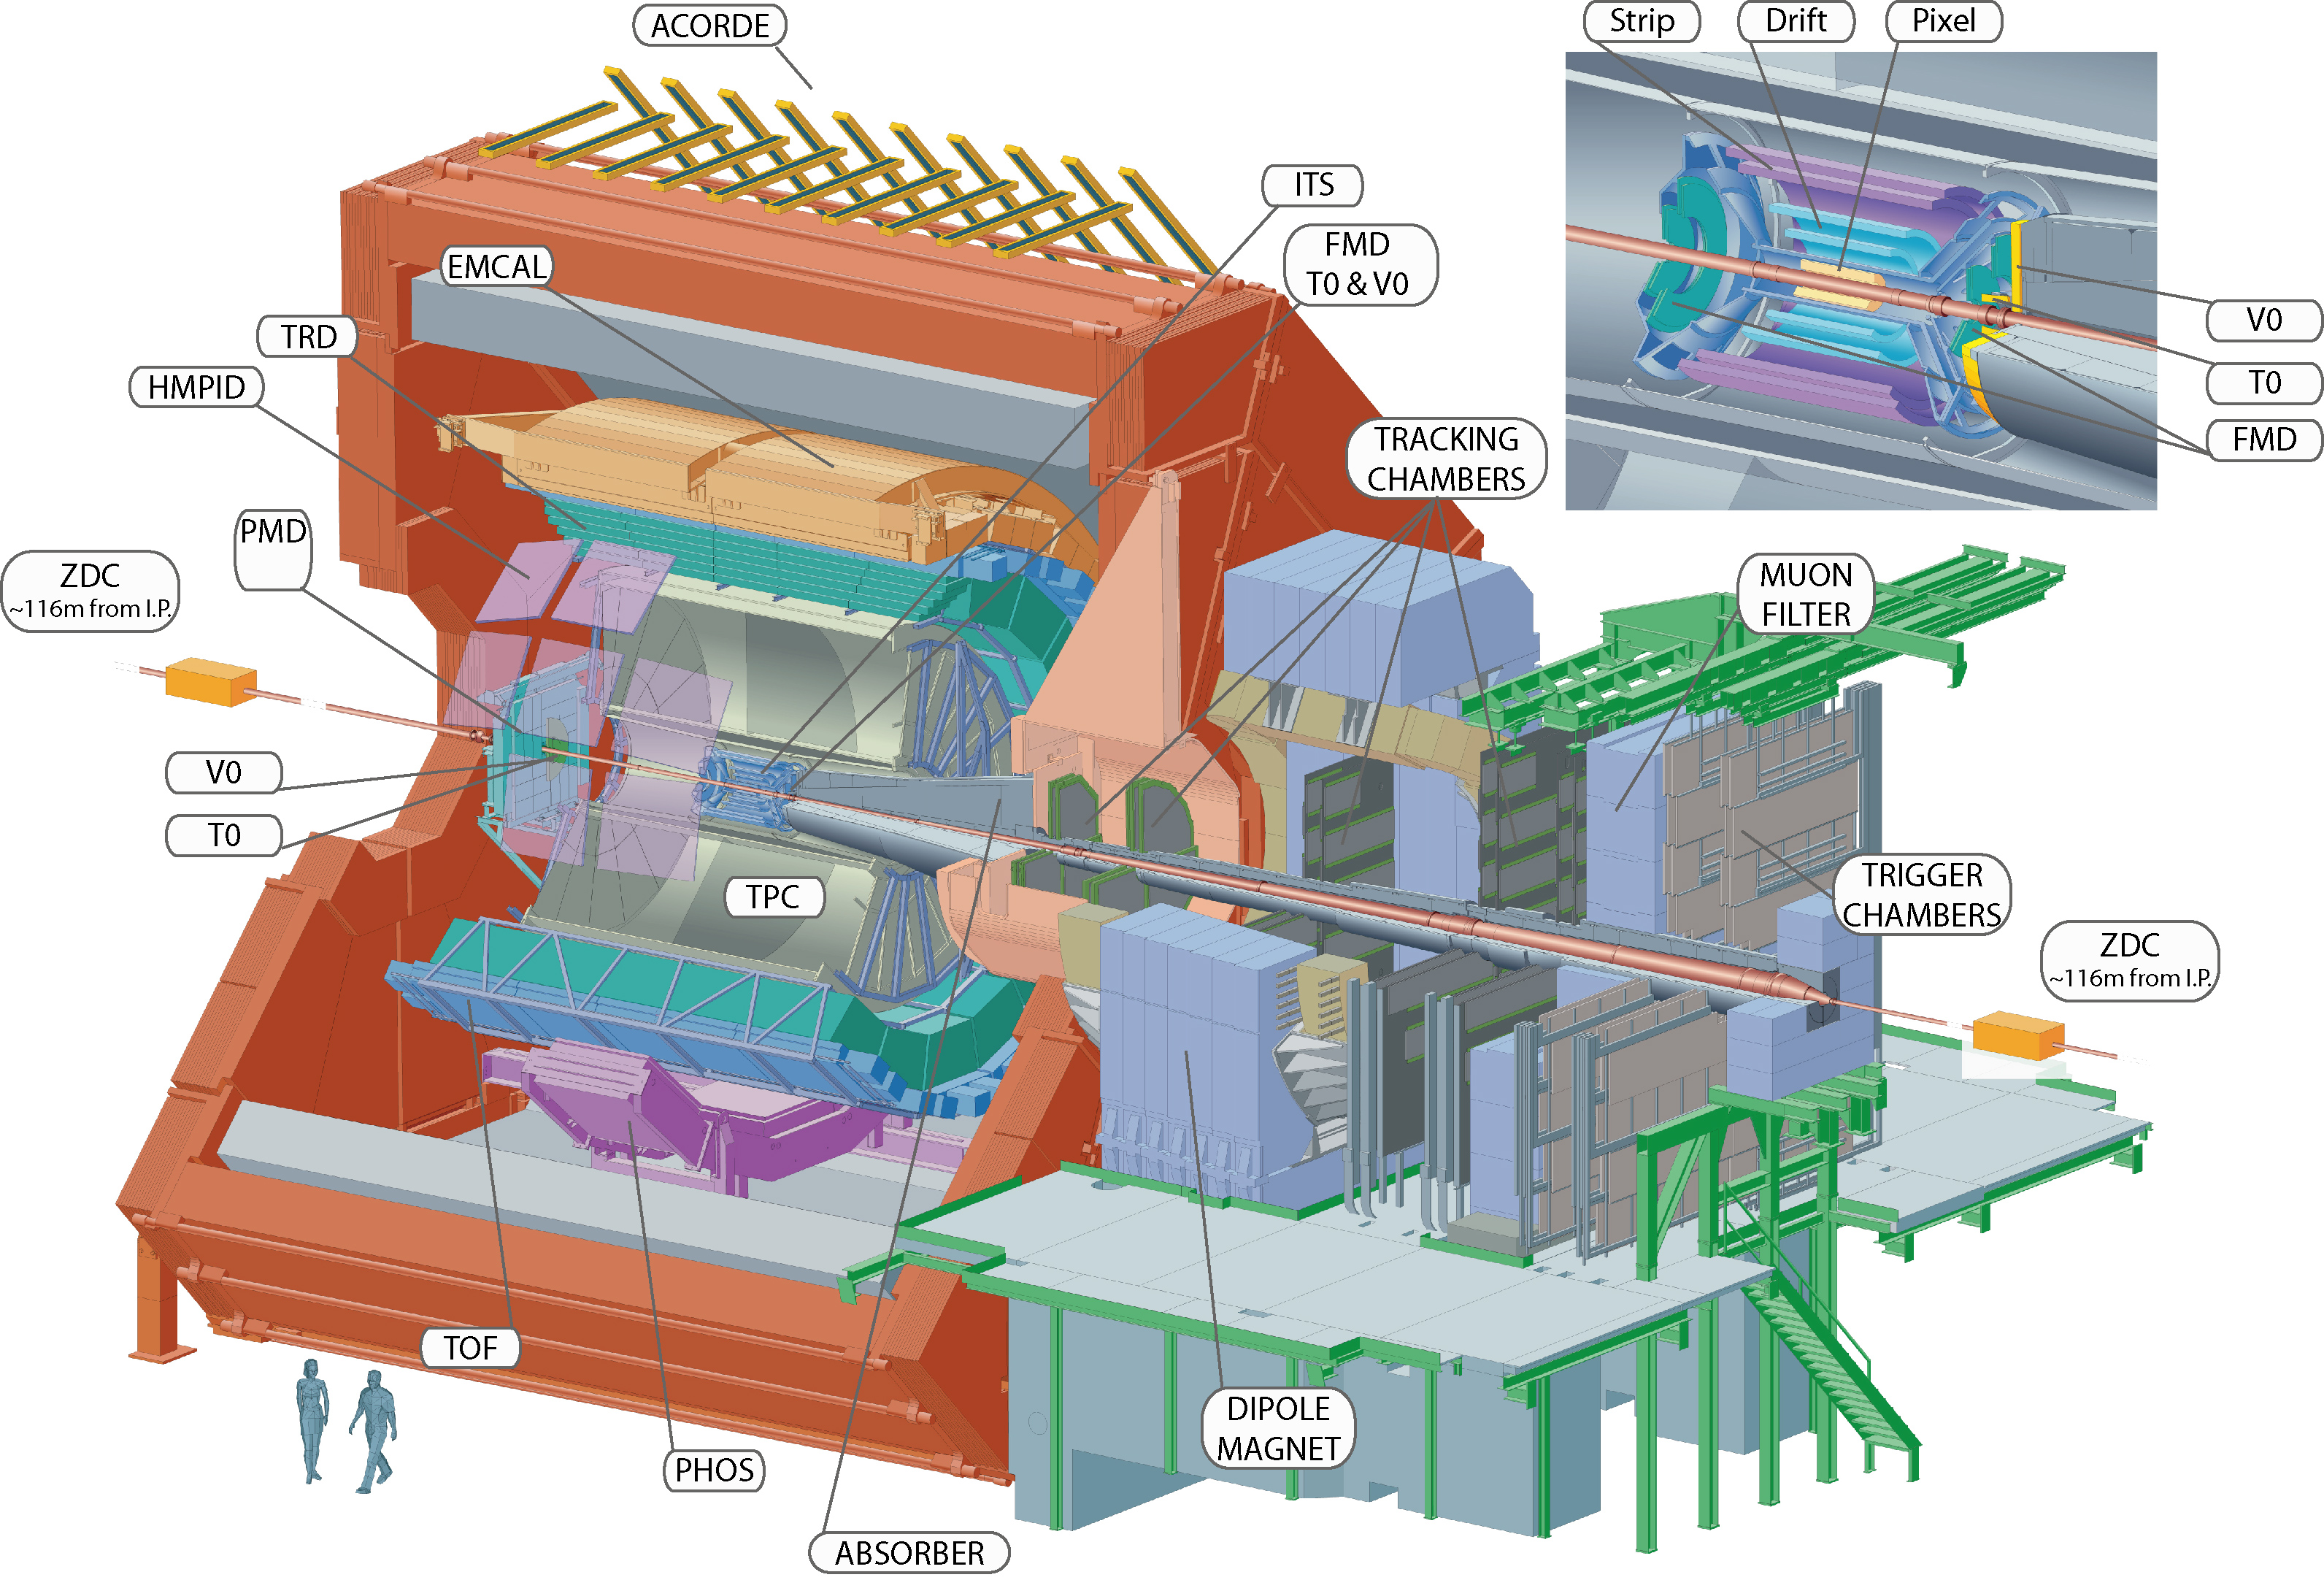
\includegraphics[width=.9\linewidth]{ALICE.jpg}
\caption{Schematische Darstellung des Querschnitts des ALICE Experiments.
\cite{WEBSITE:1}}
\label{fig:ALICE}
\end{figure}
Abbildung \ref{fig:ALICE} zeigt schematisch einen Querschnitt des ALICE Experiments. Der zylinderförmige Aufbau um das Kollisionszentrum ist typisch für Kollisionsexperimente.
\newline
Um die zentralen Detektoren herum befindet sich ein Solenoid-Magnet, der ein Magnetfeld von $0,5 \text{T}$ erzeugt, wodurch geladene Teilchen auf gekrümmte Flugbahnen gelenkt werden.
Mit Hilfe der Radien der gekrümmten Flugbahnen können geladene Teilchen identifiziert werden.
Im Folgenden werden die für diese Analyse wichtigsten Detektoren kurz eingeführt.
\newline
Das \textbf{Inner Tracking System}, kurz ITS, befindet sich am nächsten zum Strahlrohr des ALICE Experiments und besteht aus sechs Schichten.
In dieser Analyse wird das ITS zur Abschätzung des Kollisionspunktes, den primären Vertex, benutzt.
\newline
Die \textbf{Time Projection Chamber}, kurz TPC, umschließt das ITS und dient als Detektor der Spurrekonstruktion.
Geladene Teilchen hinterlassen in der TPC Spuren, anhand dieser können sie identifiziert werden.
\newline
Das \textbf{V0-Detektorsystem} besteht aus zwei einzelnen Detektoren, welche sich jeweils an einem Ende des ITS um das Strahlrohr befinden.
Messen beide V0 Detektoren eine bestimmte Mindestanzahl an Teilchen, so wird eine Aufzeichnung des Ereignisses (engl. \textit{event}) gestartet.
Die Anforderungen für die Messung eines \textit{events} werden allgemein als \textit{trigger} bezeichnet.
Dass die V0-Detektoren eine Mindestanzahl an Teilchen detektieren, entspricht einer Mindestanforderung an das \textit{event}.
Entsprechend wird diese Mindestanforderung \textit{minimum-bias trigger} und das \textit{event} \textit{minimum-bias event} genannt.
\newline
Genau wie das V0-Detektorsystem bestehen das \textbf{T0-Detektorsystem} aus zwei einzelnen Detektoren, die sich an den Enden des ITS befinden.
Die T0-Detektoren sind auf präzise Zeitmessungen spezialisiert und legen den Zeitpunkt der Kollision fest.
\newline
Das \textbf{Elektromagnetische Kalorimeter}, kurz EMCal, befindet sich am äußersten Rand des zentralen Detektors.
Da in dieser Analyse Messungen des EMCals verwendet werden, wird der Aufbau und die Funktionsweise des EMCals im folgenden Abschnitt genauer erläutert.